\begin{activity} \label{A:11.1.3} Let $f(x,y) = \sqrt{4-y^2}$ on the rectangular domain $R = [1,7] \times [-2,2]$. Partition $[1,7]$ into 3 equal length subintervals and $[-2,2]$ into 2 equal length subintervals. A table of values of $f$ at some points in $R$ is given in Table \ref{DI:11.1.TOV}, and a graph of $f$ with the indicated partitions is shown in Figure \ref{F:11.1.DI_example}.

\begin{figure}[ht]
\begin{center}
\begin{minipage}{2.5in}
\begin{center}
\begin{tabular}{|c||c|c|c|c|c|} \hline
    &$-2$   &$-1$       &$0$    &$1$        &$2$ \\ \hhline{|=|=|=|=|=|=|}
$1$ &$0$    &$\sqrt{3}$ &$2$    &$\sqrt{3}$ &$0$ \\ \hline
$2$ &$0$    &$\sqrt{3}$ &$2$    &$\sqrt{3}$ &$0$ \\ \hline
$3$ &$0$    &$\sqrt{3}$ &$2$    &$\sqrt{3}$ &$0$ \\ \hline
$4$ &$0$    &$\sqrt{3}$ &$2$    &$\sqrt{3}$ &$0$ \\ \hline
$5$ &$0$    &$\sqrt{3}$ &$2$    &$\sqrt{3}$ &$0$ \\ \hline
$6$ &$0$    &$\sqrt{3}$ &$2$    &$\sqrt{3}$ &$0$ \\ \hline
$7$ &$0$    &$\sqrt{3}$ &$2$    &$\sqrt{3}$ &$0$ \\ \hline
\end{tabular}
\end{center}
\captionof{table}{Table of values of $f(x,y) =  \sqrt{4-y^2}$.}
\label{DI:11.1.TOV}
\end{minipage} \hspace{0.5in}
\begin{minipage}{2.5in}
\begin{center}
%\resizebox{!}{1.5in}{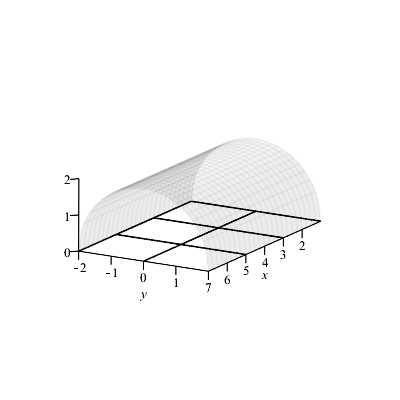
\includegraphics[trim=2cm 3.5cm 2cm 4.5cm, clip]{11_1_DI_example}}
  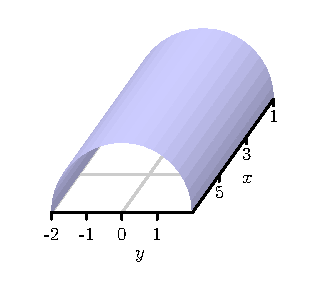
\includegraphics{figures/fig_11_1_cylinder.eps}
%crop graphics in animate trim=<left> <bottom> <right> <top>, add, clip with \includegraphics
\end{center}
\captionof{figure}{Graph of $f(x,y) =  \sqrt{4-y^2}$ on $R$.}
\label{F:11.1.DI_example}
\end{minipage}
\end{center}
\end{figure}

    \ba
    \item Outline the partition of $R$ into subrectangles on the table of values in Table \ref{DI:11.1.TOV}.



    \item Calculate the double Riemann sum using the given partition of $R$ and the values of $f$ in the upper right corner of each subrectangle.


    \item Use geometry to calculate the exact value of $\iint_R f(x,y) \, dA$ and compare it to your approximation. How could we obtain a better approximation?



    \ea

\end{activity}
\begin{smallhint}

\end{smallhint}
\begin{bighint}

\end{bighint}
\begin{activitySolution}
    \ba
    \item The endpoints of the partition of $[1,7]$ are $1$, $3$, $5$, and $7$, while the endpoints of the partition of $[-2,2]$ are $-2$, $0$, and $2$. This makes subrectangles $R_{11} = [1,3] \times [-2,0]$, $R_{21} = [3,5] \times [-2,0]$, $R_{31} = [5,7] \times [-2,0]$, $R_{12} = [1,3] \times [0,2]$, $R_{22} = [3,5] \times [0,2]$, $R_{32} = [5,7] \times [0,2]$. These subrectangles are outlined in the table below.
\begin{center}
\setlength{\unitlength}{0.8cm}
\begin{picture}(6,8)
%Horizontal lines
\put(0,0){\line(1,0){6}}
%\put(0,1){\line(1,0){6}}
%\put(0,2){\line(1,0){6}}
%\put(0,3){\line(1,0){6}}
%\put(0,4){\line(1,0){6}}
%\put(0,5){\line(1,0){6}}
%\put(0,6){\line(1,0){6}}
\put(0,7){\line(1,0){6}}
\put(0,8){\line(1,0){6}}
\put(0,2.5){\line(1,0){6}}
\put(0,4.5){\line(1,0){6}}
%Vertical lines
\put(0,0){\line(0,1){8}}
\put(1,0){\line(0,1){8}}
%\put(2,0){\line(0,1){8}}
%\put(3,0){\line(0,1){8}}
%\put(4,0){\line(0,1){8}}
%\put(5,0){\line(0,1){8}}
\put(6,0){\line(0,1){8}}
\put(3.5,0){\line(0,1){8}}
%Table entries
\put(1.2,7.4){$-2$}
\put(2.2,7.4){$-1$}
\put(3.4,7.4){$0$}
\put(4.4,7.4){$1$}
\put(5.4,7.4){$2$}
\put(0.4,6.4){$1$}
\put(1.4,6.4){$0$}
\put(2.15,6.4){$\sqrt{3}$}
\put(3.4,6.4){$2$}
\put(4.15,6.4){$\sqrt{3}$}
\put(5.4,6.4){$0$}
\put(0.4,5.4){$2$}
\put(1.4,5.4){$0$}
\put(2.15,5.4){$\sqrt{3}$}
\put(3.4,5.4){$2$}
\put(4.15,5.4){$\sqrt{3}$}
\put(5.4,5.4){$0$}
\put(0.4,4.4){$3$}
\put(1.4,4.4){$0$}
\put(2.15,4.4){$\sqrt{3}$}
\put(3.4,4.4){$2$}
\put(4.15,4.4){$\sqrt{3}$}
\put(5.4,4.4){$0$}
\put(0.4,3.4){$4$}
\put(1.4,3.4){$0$}
\put(2.15,3.4){$\sqrt{3}$}
\put(3.4,3.4){$2$}
\put(4.15,3.4){$\sqrt{3}$}
\put(5.4,3.4){$0$}
\put(0.4,2.4){$5$}
\put(1.4,2.4){$0$}
\put(2.15,2.4){$\sqrt{3}$}
\put(3.4,2.4){$2$}
\put(4.15,2.4){$\sqrt{3}$}
\put(5.4,2.4){$0$}
\put(0.4,1.4){$6$}
\put(1.4,1.4){$0$}
\put(2.15,1.4){$\sqrt{3}$}
\put(3.4,1.4){$2$}
\put(4.15,1.4){$\sqrt{3}$}
\put(5.4,1.4){$0$}
\put(0.4,0.4){$7$}
\put(1.4,0.4){$0$}
\put(2.15,0.4){$\sqrt{3}$}
\put(3.4,0.4){$2$}
\put(4.15,0.4){$\sqrt{3}$}
\put(5.4,0.4){$0$}
\end{picture}
\end{center}


    \item Choosing points in the upper right corner of each subrectangle gives us $(x_{11}^*, y_{11}^*) = (3,0)$, $(x_{21}^*, y_{21}^*) = (5,0)$, $(x_{31}^*, y_{31}^*) = (7,0)$, $(x_{12}^*, y_{12}^*) = (3,2)$, $(x_{22}^*, y_{22}^*) = (5,2)$, and $(x_{32}^*, y_{32}^*) = (7,2)$. So 
\begin{align*}
\sum_{j=1}^n \sum_{i=1}^m f\left(x_{ij}^*, y_{ij}^*\right) \cdot \Delta A &= f(3,0)(4) + f(5,0)(4) + f(7,0)(4) + f(3,2)(4) + f(5,3)(4) + f(7,2)(4) \\
	&= 24.
\end{align*}

    \item Since the cross sections parallel to the $yz$-plane are semi-circles of radius 2, we can multiply the area of a cross section by the width to obtain the volume. So the exact volume of this object is $4 \pi (6) = 24 \pi$. We could get a better approximation by using finer partitions.  


    \ea
\end{activitySolution}
\aftera
